\subsection{Analytic description}
To describe the non-Euclidean geometries analytically, we will follow the approach given by \cite{Szirmay-Kalos2022}.
This approach allows us to view the points of a 3-dimensional non-Euclidean space as a subset of the 4-dimensional \textit{embedding space}.
Since imagining the fourth dimension is not something particularly easy, we will be decreasing the dimensionality whenever we give examples.

The elliptic space can be modeled as a unit 3-sphere, \textit{embedded} in a 4-dimensional Euclidean space.
By saying that a space is embedded in another, we mean that the embedded space inherits the distance from the embedding space.
In this case, the spherical distance, given by $ds^2 = dx^2 + dy^2 + dz^2 + dw^2$ is derived from the Euclidean distance.
This is similar to how we may model the 2-dimensional elliptic space as a sphere, where lines are identified with great circles.
The inner product of two vectors $u$ and $v$ in the Euclidean space is given by
$$ \langle u, v \rangle_E  = u_xv_x + u_yv_y + u_zv_z + u_wv_w.$$
Thus, we can define that a point $p$ belongs to the elliptic geometry if
$$ \langle p, p \rangle_E = 1.$$

The model that we use for the hyperbolic geometry is the so-called \textit{hyperboloid model}.
In this model, points $p$ of the hyperbolic space satisfy the equation
$$p_x^2 + p_y^2 + p_z^2 - p_w^2 = -1,$$
with $p_w > 0$.
The set of these points creates the upper sheet of a hyperboloid, which could be visualized as shown in \autoref{fig:hyperboloid} if the embedding space was Euclidean.
\begin{figure}[h]
    \centering
    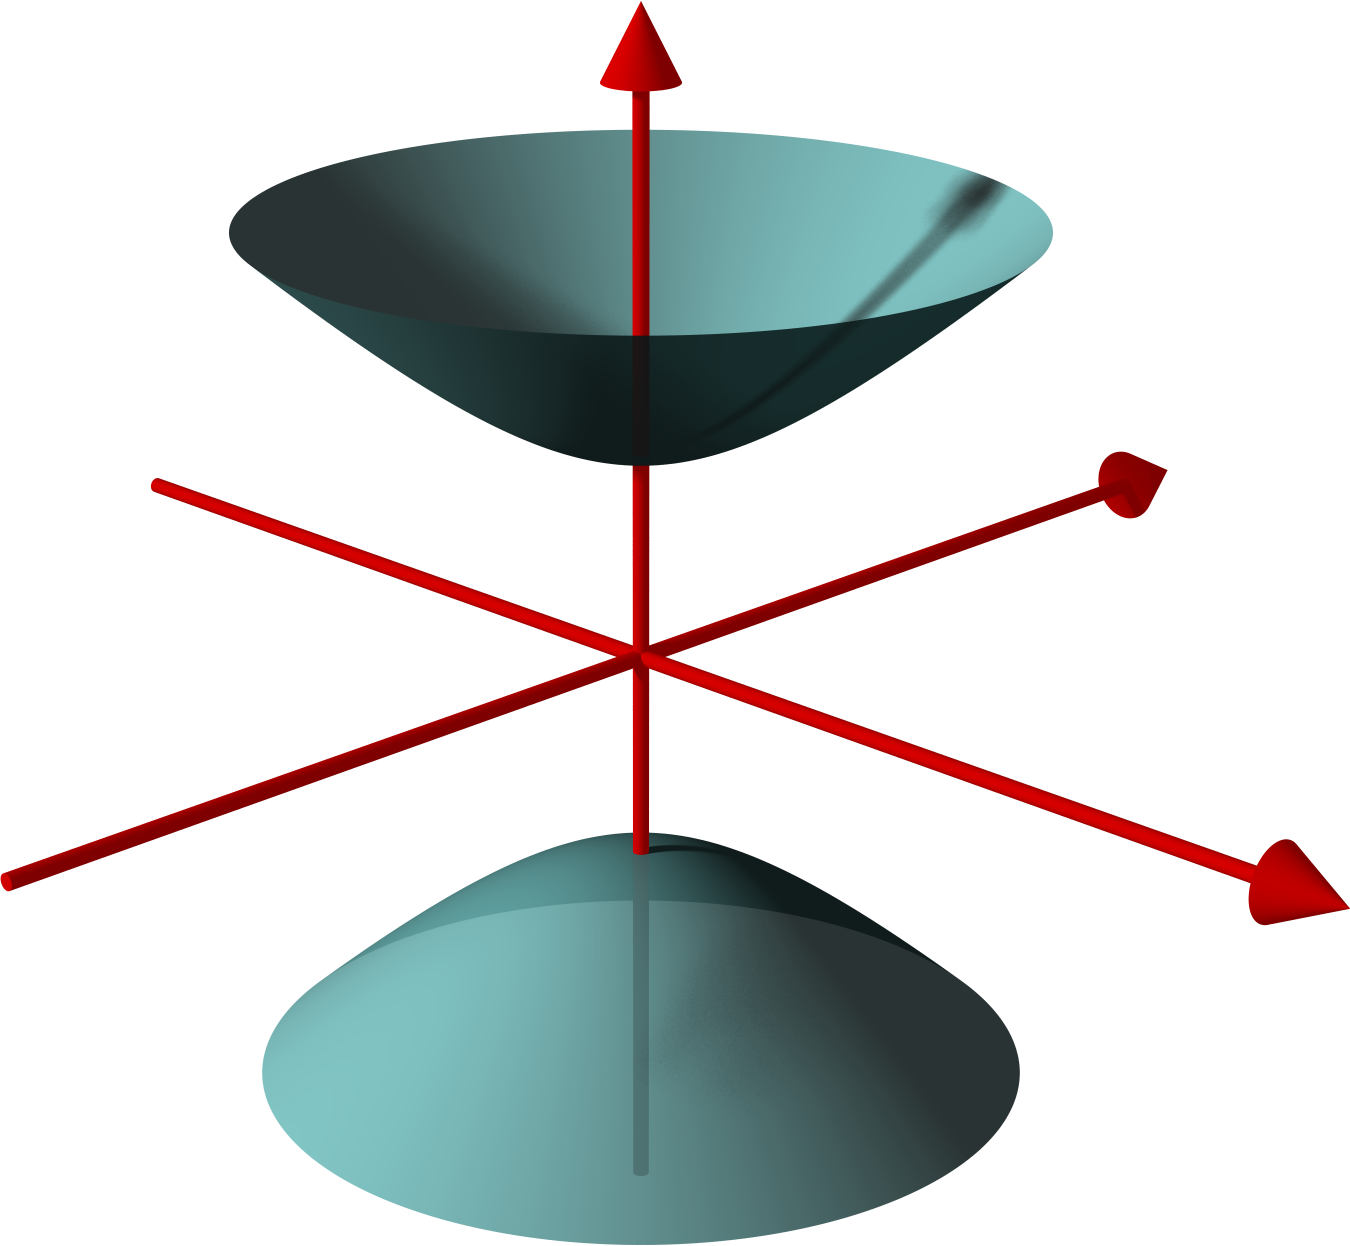
\includegraphics[width=0.4\textwidth]{chapters/theoretical_foundations/sections/non-eudlidean-spaces/resources/hyperboloid.png}
    \caption{2-dimensional hyperboloid embedded in Euclidean space}
    \label{fig:hyperboloid}
\end{figure}
However, the hyperbolic space is not embedded in the Euclidean space, but in the \textit{Minkowski space} instead.
In the Minkowski space, the inner product of vectors $u$, $v$ is given by the Lorentzian inner product:
$$\langle u, v \rangle_L = u_xv_x + u_yv_y + u_zv_z - u_wv_w.$$
Thus, the points $p$ belonging to the hyperbolic geometry satisfy the equation
$$\langle p, p \rangle_L = -1.$$
It could be interpreted that they are located on a sphere with a radius of imaginary length $\sqrt{-1}$ (and hence are equidistant from the origin).

To build a unified framework for discussing both types of geometries, we introduce the notion of \textit{sign of curvature}, $\mathcal{L}$, that attains the value $+1$ for spherical, and $-1$ for hyperbolic space.
We also define the generalized inner product
\begin{equation} \label{eq:gen-inner-prod}
    \langle u, v \rangle = u_xv_x + u_yv_y + u_zv_z + \mathcal{L}u_wv_w.
\end{equation}

